\documentclass[10pt]{article}
\usepackage[utf8]{inputenc}
\usepackage[english]{babel}
\usepackage{amsmath, amssymb}
\usepackage{xcolor}
\usepackage{geometry}
\geometry{letterpaper, margin=1in}
\usepackage{graphicx}
\usepackage{float}
\usepackage{array}
\usepackage{booktabs}
\usepackage{colortbl}
\usepackage{caption}
\usepackage{tocloft}
\usepackage[colorlinks=true, linkcolor=black, urlcolor=black, citecolor=black]{hyperref}
\usepackage{hwemoji}
%%%%%%%%%%%%%%%%%%%%%%%%%%%%%%%%%%%%%%%%%%%%%%%%%%%%%%%%%%%%%%%%%%%%%%%%%%%%%%%%%%%%%%%%%%%%%
\title{Universidad Panamericana \\ Master's in Data Sciences \\ Natural Language Processing \\ 
    \vspace{0.5cm} Final Project: \textit{Sentiment Analysis of FIFA World Cup Tweets}}
\author{Enrique Ulises Báez Gómez Tagle}
\date{\today}
%%%%%%%%%%%%%%%%%%%%%%%%%%%%%%%%%%%%%%%%%%%%%%%%%%%%%%%%%%%%%%%%%%%%%%%%%%%%%%%%%%%%%%%%%%%%%
\begin{document}
\maketitle
\tableofcontents
\newpage
%%%%%%%%%%%%%%%%%%%%%%%%%%%%%%%%%%%%%%%%%%%%%%%%%%%%%%%%%%%%%%%%%%%%%%%%%%%%%%%%%%%%%%%%%%%%%
\section*{Abstract}
This project aims to perform sentiment analysis on tweets related to the FIFA World Cup 2022 using both traditional machine learning and deep learning models. 
The dataset contains 30,000 tweets collected on the first day of the tournament using the \texttt{Snscrape} library and pre-labeled with the\\ \texttt{cardiffnlp/twitter-roberta-base-sentiment-latest} model from Hugging Face.
We compare classical approaches (e.g., Logistic Regression, SVM) using TF-IDF features against neural architectures such as LSTM, CNN, and Transformer-based models. 
Evaluation metrics include Accuracy, Precision, Recall, and F1-score. The results highlight how deep learning models outperform traditional ones in handling contextual nuances of tweets.
%%%%%%%%%%%%%%%%%%%%%%%%%%%%%%%%%%%%%%%%%%%%%%%%%%%%%%%%%%%%%%%%%%%%%%%%%%%%%%%%%%%%%%%%%%%%%
\section{Introduction}
The FIFA World Cup is one of the largest and most influential sporting events worldwide, attracting billions of viewers and generating massive engagement across digital platforms. During the 2022 edition in Qatar, social media—especially Twitter—became a real-time forum for fans to express opinions, emotions, and reactions to matches, players, and events. This global activity creates a rich source of textual data that can be leveraged to analyze public sentiment and collective emotional dynamics surrounding major sports events.

Understanding the sentiment behind these tweets is important for several reasons. First, it provides valuable insights into fan behavior, public perception of teams and players, and the emotional impact of sporting events on different audiences. Second, sentiment analysis can assist broadcasters, sponsors, and organizations such as FIFA in gauging audience engagement and reputation trends. Finally, from a data science perspective, it represents a challenging Natural Language Processing (NLP) problem due to the informal, multilingual, and often sarcastic nature of social media text \cite{ref1, ref2, ref3}.

Sentiment analysis, or opinion mining, aims to classify text into categories such as positive, negative, or neutral, based on the emotional tone conveyed by users. Previous research has explored a range of approaches—from traditional machine learning models such as Logistic Regression, Support Vector Machines (SVM), and Random Forests \cite{ref1} to deep learning architectures like Convolutional Neural Networks (CNN) and Long Short-Term Memory (LSTM) networks \cite{ref2}. More recently, transformer-based models such as BERT and RoBERTa have achieved state-of-the-art results in sentiment classification tasks on Twitter data \cite{ref3, ref4}.

Building upon this body of work, this project focuses on the sentiment analysis of tweets related to the 2022 FIFA World Cup. Tweets are categorized into three sentiment classes—positive, neutral, and negative—using both traditional machine learning and modern deep learning models. The goal is to evaluate how different text representations and architectures perform in understanding contextual nuances, emotion, and sarcasm in sports-related tweets. Through this comparison, the study contributes to the broader understanding of how NLP techniques can extract meaningful insights from real-world social media discourse.
%%%%%%%%%%%%%%%%%%%%%%%%%%%%%%%%%%%%%%%%%%%%%%%%%%%%%%%%%%%%%%%%%%%%%%%%%%%%%%%%%%%%%%%%%%%%%
\section{Related Work}
Previous research on sentiment analysis of sports-related tweets has evolved significantly over the past decade, progressing from traditional machine learning approaches to deep neural and transformer-based architectures. 

Early works (2016–2018) commonly employed statistical text representations such as Bag-of-Words and TF-IDF combined with models like Logistic Regression, Linear SVC, Random Forest and Bayesian Logistic Regression. For instance, Barnaghi et al. \cite{ref1} analyzed FIFA World Cup 2014 tweets using TF-IDF with Bayesian Logistic Regression, achieving competitive accuracy but later works noted limitations in capturing sarcasm and emoji-driven sentiment.

From 2018 onward, deep learning architectures such as CNN and LSTM began outperforming traditional classifiers in sentiment analysis tasks. Venkatesh et al. \cite{ref2} proposed a CNN-LSTM hybrid for classifying sports tweets, demonstrating that combining convolutional and recurrent layers improved contextual understanding.

The next major shift came with transformer-based models like BERT and RoBERTa, which leverage self-attention mechanisms and large-scale pretraining. Barbieri et al. \cite{ref3} introduced the TweetEval benchmark, fine-tuning RoBERTa for multiple Twitter NLP tasks and achieving state-of-the-art sentiment accuracy. More recent studies (2021–2025) fine-tuned RoBERTa specifically on sports tweets \cite{ref4}, reporting superior F1-scores and robustness compared to CNN and LSTM models.

This project builds upon these advancements by directly comparing traditional machine learning models (Logistic Regression, Linear SVC, Random Forest) with deep learning architectures (LSTM, CNN) and transformer-based methods (RoBERTa as both feature extractor and fine-tuned model) on FIFA World Cup 2022 tweets. By systematically evaluating across these paradigms, this work highlights the evolution of sentiment analysis methods and quantifies the contextual advantages of transformer-based approaches for real-world, event-driven social media data.
%%%%%%%%%%%%%%%%%%%%%%%%%%%%%%%%%%%%%%%%%%%%%%%%%%%%%%%%%%%%%%%%%%%%%%%%%%%%%%%%%%%%%%%%%%%%%
\section{Methodology}

\subsection{Dataset Description}
The dataset used in this project is titled \textbf{"FIFA World Cup 2022 Tweets"}, consisting of approximately \textbf{30,000 tweets} collected during the first day of the tournament in Qatar 2022.

Data was obtained using the \texttt{Snscrape} library for scraping and labeled automatically with the pre-trained RoBERTa-based sentiment model
\href{https://huggingface.co/cardiffnlp/twitter-roberta-base-sentiment-latest}{\texttt{cardiffnlp/twitter-roberta-base-sentiment-latest}} from Hugging Face.
The dataset is stored as a CSV file named \texttt{fifa\_world\_cup\_2022\_tweets.csv} and contains the following columns:
\begin{itemize}
    \item \textbf{Date Created}: Timestamp of tweet publication.
    \item \textbf{Number of Likes}: Engagement measure.
    \item \textbf{Source of Tweet}: Platform or device used to post.
    \item \textbf{Tweet}: Raw text content of the tweet.
    \item \textbf{Sentiment}: Pre-assigned label (Positive, Neutral, or Negative).
\end{itemize}
The dataset is publicly available under the \textbf{CC0 1.0 Universal (Public Domain)} license, allowing unrestricted reuse and modification.
%%%%%%%%%%%%%%%%%%%%%%%%%%%%%%%%%%%%%%%%%%%%%%%%%%%%%%%%%%%%%%%%%%%%%%%%%%%%%%%%%%%%%%%%%%%%%
\subsection{Preprocessing}
The preprocessing pipeline was implemented in Python using regular expressions to robustly clean and normalize tweet text while preserving sentiment cues.
All text is first converted to lowercase. Mentions (e.g., @usernames) are replaced with the token \texttt{USR}, and URLs with \texttt{URL}.
Hashtags are preserved as semantic tokens by replacing the symbol \# with the prefix \texttt{hash\_}.
Additionally, a curated list of emoticons (e.g., \texttt{:-)}, \texttt{XD}) and emojis (e.g., 😊, 🔥, 😭) is kept intact to retain emotional context.
A whitelist of characters ensures that only meaningful alphanumeric and sentiment-relevant symbols (e.g., \texttt{! ? ( ) : -}) are preserved, avoiding the loss of informal markers common in social media text.
Finally, redundant spaces are removed, resulting in clean and normalized text ready for tokenization and embedding generation.
%%%%%%%%%%%%%%%%%%%%%%%%%%%%%%%%%%%%%%%%%%%%%%%%%%%%%%%%%%%%%%%%%%%%%%%%%%%%%%%%%%%%%%%%%%%%%
\subsection{Feature Extraction}
After preprocessing, the data was split with a stratified 80/20 train--test partition (\texttt{random\_state=42}).

\paragraph{Statistical representations.}
For traditional ML models, we use a TF--IDF vectorizer with \textit{max\_features} $=50{,}000$, n-grams $(1,3)$, \textit{min\_df}$=2$, and English stopwords. The resulting sparse matrix feeds Logistic Regression, Linear SVM, and Random Forest.

\paragraph{Semantic representations (word embeddings).}
For sequence models, we use \textbf{GloVe-Twitter-200} (via \texttt{gensim}). A Keras \textit{Tokenizer} (\textit{num\_words}$=50{,}000$, explicit \texttt{<OOV>}) builds the vocabulary; sequences are padded/truncated to $L=180$. The embedding matrix is aligned to this vocab, with zero vector at the padding index and the \texttt{<OOV>} vector set to the mean of known embeddings.

\paragraph{Transformer representations.}
We employ \textbf{cardiffnlp/twitter-roberta-base-sentiment-latest} in two modes:
\begin{enumerate}
  \item \textbf{Feature extractor:} we freeze the backbone and compute sentence embeddings with masked mean-pooling over the last hidden states (max length 96 tokens, batch size 64, \texttt{no\_grad}). Train/test embeddings are cached to \texttt{.npy}.
  \item \textbf{Fine-tuning:} we tokenize to 128 tokens and train a classification head end-to-end using \texttt{Trainer}.
\end{enumerate}
%%%%%%%%%%%%%%%%%%%%%%%%%%%%%%%%%%%%%%%%%%%%%%%%%%%%%%%%%%%%%%%%%%%%%%%%%%%%%%%%%%%%%%%%%%%%%
\subsection{Modeling}

\subsubsection{Traditional Machine Learning Models}
\textbf{Logistic Regression (TF--IDF).} Multinomial Logistic Regression with \texttt{max\_iter}$=2000$, \texttt{C}$=1.0$, and \textit{class\_weight}=\texttt{balanced}.\\
\textbf{Linear SVM (TF--IDF).} \texttt{LinearSVC} with \texttt{C}$=1.0$ (hinge loss).\\
\textbf{Random Forest (TF--IDF).} \texttt{n\_estimators}$=400$, \texttt{max\_depth=None}, \texttt{min\_samples\_split}$=2$,\\
\textit{class\_weight}=\texttt{balanced\_subsample}, \texttt{n\_jobs}$=-1$.\\
All models are trained on the TF--IDF features and evaluated with macro-averaged accuracy, precision, recall, and F1.

\subsubsection{Deep Learning Models}

\paragraph{CNN with Squeeze-and-Excitation and attention.}
\texttt{TextCNN\_TwitterSE\_Attn} architecture:
\begin{itemize}
  \item \textbf{Input:} token indices ($L=180$) with \texttt{SpatialDropout1D}(0.2).
  \item \textbf{Embedding:} GloVe-Twitter-200 matrix (frozen in Stage~1; unfrozen in Stage~2).
  \item \textbf{Trunk:} five \texttt{Conv1D} branches (128 filters; kernel sizes $\{2,3,4,5,7\}$), each followed by \texttt{BatchNorm} and \texttt{ReLU}.
  \item \textbf{SE-block:} channel-wise recalibration with reduction ratio $r=8$.
  \item \textbf{Attention pooling:} per branch, we concatenate global max-pooling, global average-pooling, and a softmax-weighted sum across time.
  \item \textbf{Head:} concatenation $\rightarrow$ \texttt{Dropout}(0.4) $\rightarrow$ \texttt{Dense}(192, ReLU, L2=$10^{-4}$) $\rightarrow$ \texttt{Dropout}(0.4) $\rightarrow$ \texttt{Dense}(\#classes, softmax).
  \item \textbf{Training:} \texttt{sparse\_categorical\_crossentropy}, \texttt{Adam}. \textit{Stage 1}: \texttt{lr}$=10^{-3}$, batch 128, val split 0.1, \texttt{EarlyStopping(patience=3)} + \texttt{ReduceLROnPlateau}(factor 0.5, patience 2, \texttt{min\_lr}$=10^{-5}$).
        \textit{Stage 2}: unfreeze embeddings and add class weights, \texttt{lr}$=10^{-4}$, \texttt{clipnorm}$=1.0$.
        \textit{Stage 3}: \texttt{CosineDecayRestarts} with initial \texttt{lr}$=5\!\times\!10^{-5}$, batch 64; \texttt{EarlyStopping} only.
\end{itemize}

\paragraph{BiLSTM with attention.}
\texttt{BiLSTM\_Attn} architecture:
\begin{itemize}
  \item \textbf{Input/Embedding:} same as CNN (GloVe embeddings, $L=180$, \texttt{mask\_zero}).
  \item \textbf{Trunk:} \texttt{SpatialDropout1D}(0.2) $\rightarrow$ \texttt{BiLSTM}(96, \texttt{return\_sequences}) $\rightarrow$ \texttt{BiLSTM}(64, \texttt{return\_sequences}); no recurrent dropout in our runs.
  \item \textbf{Attention pooling:} tanh projection $\rightarrow$ 1D score $\rightarrow$ temporal softmax; we concatenate attention-weighted sum with global max/avg pooling.
  \item \textbf{Head:} \texttt{Dropout}(0.4) $\rightarrow$ \texttt{Dense}(128, ReLU, L2=$10^{-4}$) $\rightarrow$ \texttt{Dropout}(0.4) $\rightarrow$ \texttt{Dense}(\#classes, softmax).
  \item \textbf{Training:} three stages mirroring the CNN: Stage~1 \texttt{Adam} (\texttt{lr}$=10^{-3}$); Stage~2 unfreezes embeddings and adds class weights with \texttt{Adam} (\texttt{lr}$=10^{-4}$, \texttt{clipnorm}$=1.0$); Stage~3 uses \texttt{CosineDecayRestarts} (\texttt{lr}$=5\!\times\!10^{-5}$).
\end{itemize}

\paragraph{Transformers (RoBERTa).}
\begin{itemize}
  \item \textbf{Feature extractor + heads:} with the backbone frozen, we compute mean-pooled embeddings (96 tokens). On top, we train (i) Logistic Regression (\texttt{max\_iter}$=2000$, \texttt{C}$=1.0$) and (ii) LinearSVC (\texttt{C}$=1.0$).
  \item \textbf{Fine-tuning:} \texttt{AutoModelForSequenceClassification} with explicit \texttt{id2label}/\texttt{label2id}; tokenization to 128 tokens.
        \texttt{TrainingArguments}: \texttt{learning\_rate}$=2\cdot10^{-5}$, \texttt{per\_device\_train\_batch\_size}$=16$, \texttt{per\_device\_eval\_batch\_size}$=32$, \texttt{num\_train\_epochs}$=3$, \texttt{weight\_decay}$=0.01$, \texttt{save\_total\_limit}$=1$, \texttt{report\_to=none}. We report macro accuracy, precision, recall, and F1.
\end{itemize}

\paragraph{Ensemble.}
We aggregate per-example predictions using two strategies: (i) \textbf{weighted voting} with fixed weights $\{w_{\text{RoBERTa}}=0.90,\,w_{\text{BiLSTM}}=0.76,\,w_{\text{CNN}}=0.75\}$ and a tie-breaker that favors RoBERTa; and (ii) \textbf{majority voting} (three equal votes with the same tie-break rule). We report both and retain the one with the best macro F1.
%%%%%%%%%%%%%%%%%%%%%%%%%%%%%%%%%%%%%%%%%%%%%%%%%%%%%%%%%%%%%%%%%%%%%%%%%%%%%%%%%%%%%%%%%%%%%
\section{Experiments and Results}

\subsection{Evaluation Metrics}
We evaluate models with \emph{accuracy}, \emph{precision}, \emph{recall}, and \emph{F1-score}. Let $\{(x_i,y_i)\}_{i=1}^N$ be labeled examples with $y_i \in \mathcal{C}=\{\texttt{negative},\texttt{neutral},\texttt{positive}\}$ and predictions $\hat{y}_i$.

\paragraph{Accuracy.}
\[
\mathrm{Acc}=\frac{1}{N}\sum_{i=1}^{N}\mathbf{1}\{y_i=\hat{y}_i\}.
\]

\paragraph{Per-class precision/recall/F1.}
For each class $c\in\mathcal{C}$, define true positives $\mathrm{TP}_c$, false positives $\mathrm{FP}_c$, and false negatives $\mathrm{FN}_c$. Then
\[
\mathrm{Prec}_c=\frac{\mathrm{TP}_c}{\mathrm{TP}_c+\mathrm{FP}_c},\quad
\mathrm{Rec}_c=\frac{\mathrm{TP}_c}{\mathrm{TP}_c+\mathrm{FN}_c},\quad
\mathrm{F1}_c= \frac{2\,\mathrm{Prec}_c\,\mathrm{Rec}_c}{\mathrm{Prec}_c+\mathrm{Rec}_c}.
\]

\paragraph{Macro-averaging.}
To avoid dominance by frequent classes, we report \emph{macro} metrics:
\[
\mathrm{Prec}_{\mathrm{macro}}=\frac{1}{|\mathcal{C}|}\sum_{c\in\mathcal{C}} \mathrm{Prec}_c,\quad
\mathrm{Rec}_{\mathrm{macro}}=\frac{1}{|\mathcal{C}|}\sum_{c\in\mathcal{C}} \mathrm{Rec}_c,\quad
\mathrm{F1}_{\mathrm{macro}}=\frac{1}{|\mathcal{C}|}\sum_{c\in\mathcal{C}} \mathrm{F1}_c.
\]
All metrics are computed with \texttt{scikit-learn} using the label order \texttt{[negative, neutral, positive]} and \texttt{zero\_division=0}. Confusion matrices follow the same class order.
%%%%%%%%%%%%%%%%%%%%%%%%%%%%%%%%%%%%%%%%%%%%%%%%%%%%%%%%%%%%%%%%%%%%%%%%%%%%%%%%%%%%%%%%%%%%%
\subsection{Results Comparison}
\paragraph{Model leaderboard.}
We compare traditional, deep, and transformer-based models on the test split. Table~\ref{tab:model-comparison} summarizes macro metrics; Figure~\ref{fig:model-f1-comparison} visualizes macro-F1 across models.

\begin{table}[H]
  \centering
  \caption{Model comparison on the test set. Macro-averaged metrics; higher is better.}
  \label{tab:model-comparison}
  \begin{tabular}{lrrrr}
\toprule
Model & Accuracy & Precision & Recall & F1 \\
\midrule
RoBERTa fine-tuned (twitter-roberta-base-sentiment-latest) & 0.897800 & 0.897500 & 0.901100 & 0.899000 \\
RoBERTa feature extractor (LogReg head) & 0.886900 & 0.889200 & 0.889000 & 0.889100 \\
RoBERTa feature extractor (LinearSVC head) & 0.884200 & 0.886700 & 0.886100 & 0.886300 \\
Ensemble (Weighted Voting) & 0.809000 & 0.806300 & 0.815200 & 0.809000 \\
Ensemble (Majority Voting) & 0.809000 & 0.806300 & 0.815200 & 0.809000 \\
BiLSTM+Attention (GloVe-Twitter) & 0.764100 & 0.762100 & 0.769300 & 0.764200 \\
CNN (Twitter SE+Attn) & 0.759200 & 0.757100 & 0.766900 & 0.759300 \\
Logistic Regression (TF-IDF) & 0.706800 & 0.705000 & 0.711900 & 0.707800 \\
LinearSVC (TF-IDF) & 0.698600 & 0.700100 & 0.699000 & 0.699400 \\
RandomForest (TF-IDF) & 0.677300 & 0.686900 & 0.671900 & 0.677400 \\
\bottomrule
\end{tabular}

\end{table}

\begin{figure}[H]
  \centering
  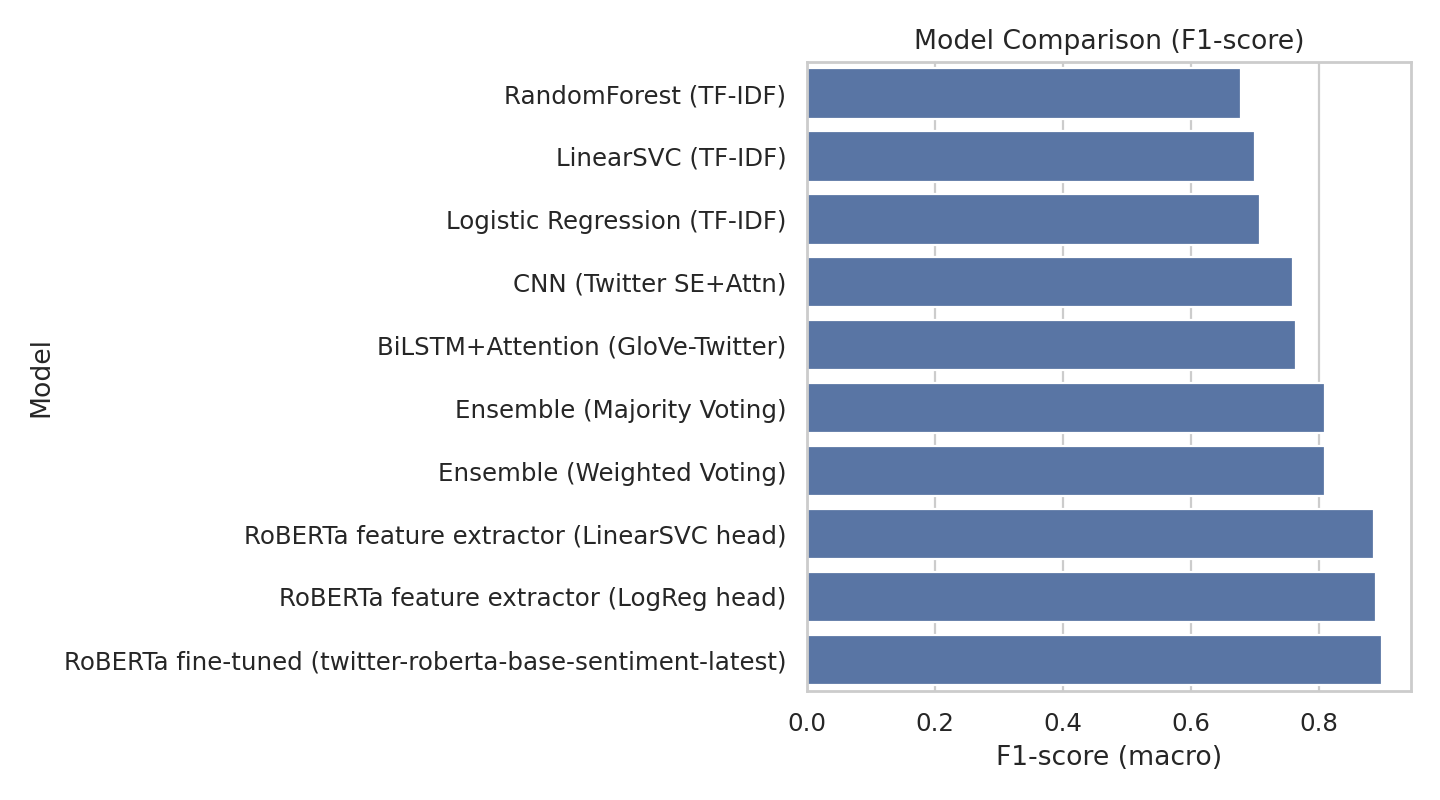
\includegraphics[width=.82\linewidth]{../SCRITPS/artifacts/figures/model_f1_comparison.png}
  \caption{Macro-F1 across all models.}
  \label{fig:model-f1-comparison}
\end{figure}

\paragraph{Per-class analysis.}
For the best model (top row in Table~\ref{tab:model-comparison}), we report its confusion matrix and per-class metrics:
\begin{figure}[H]
  \centering
  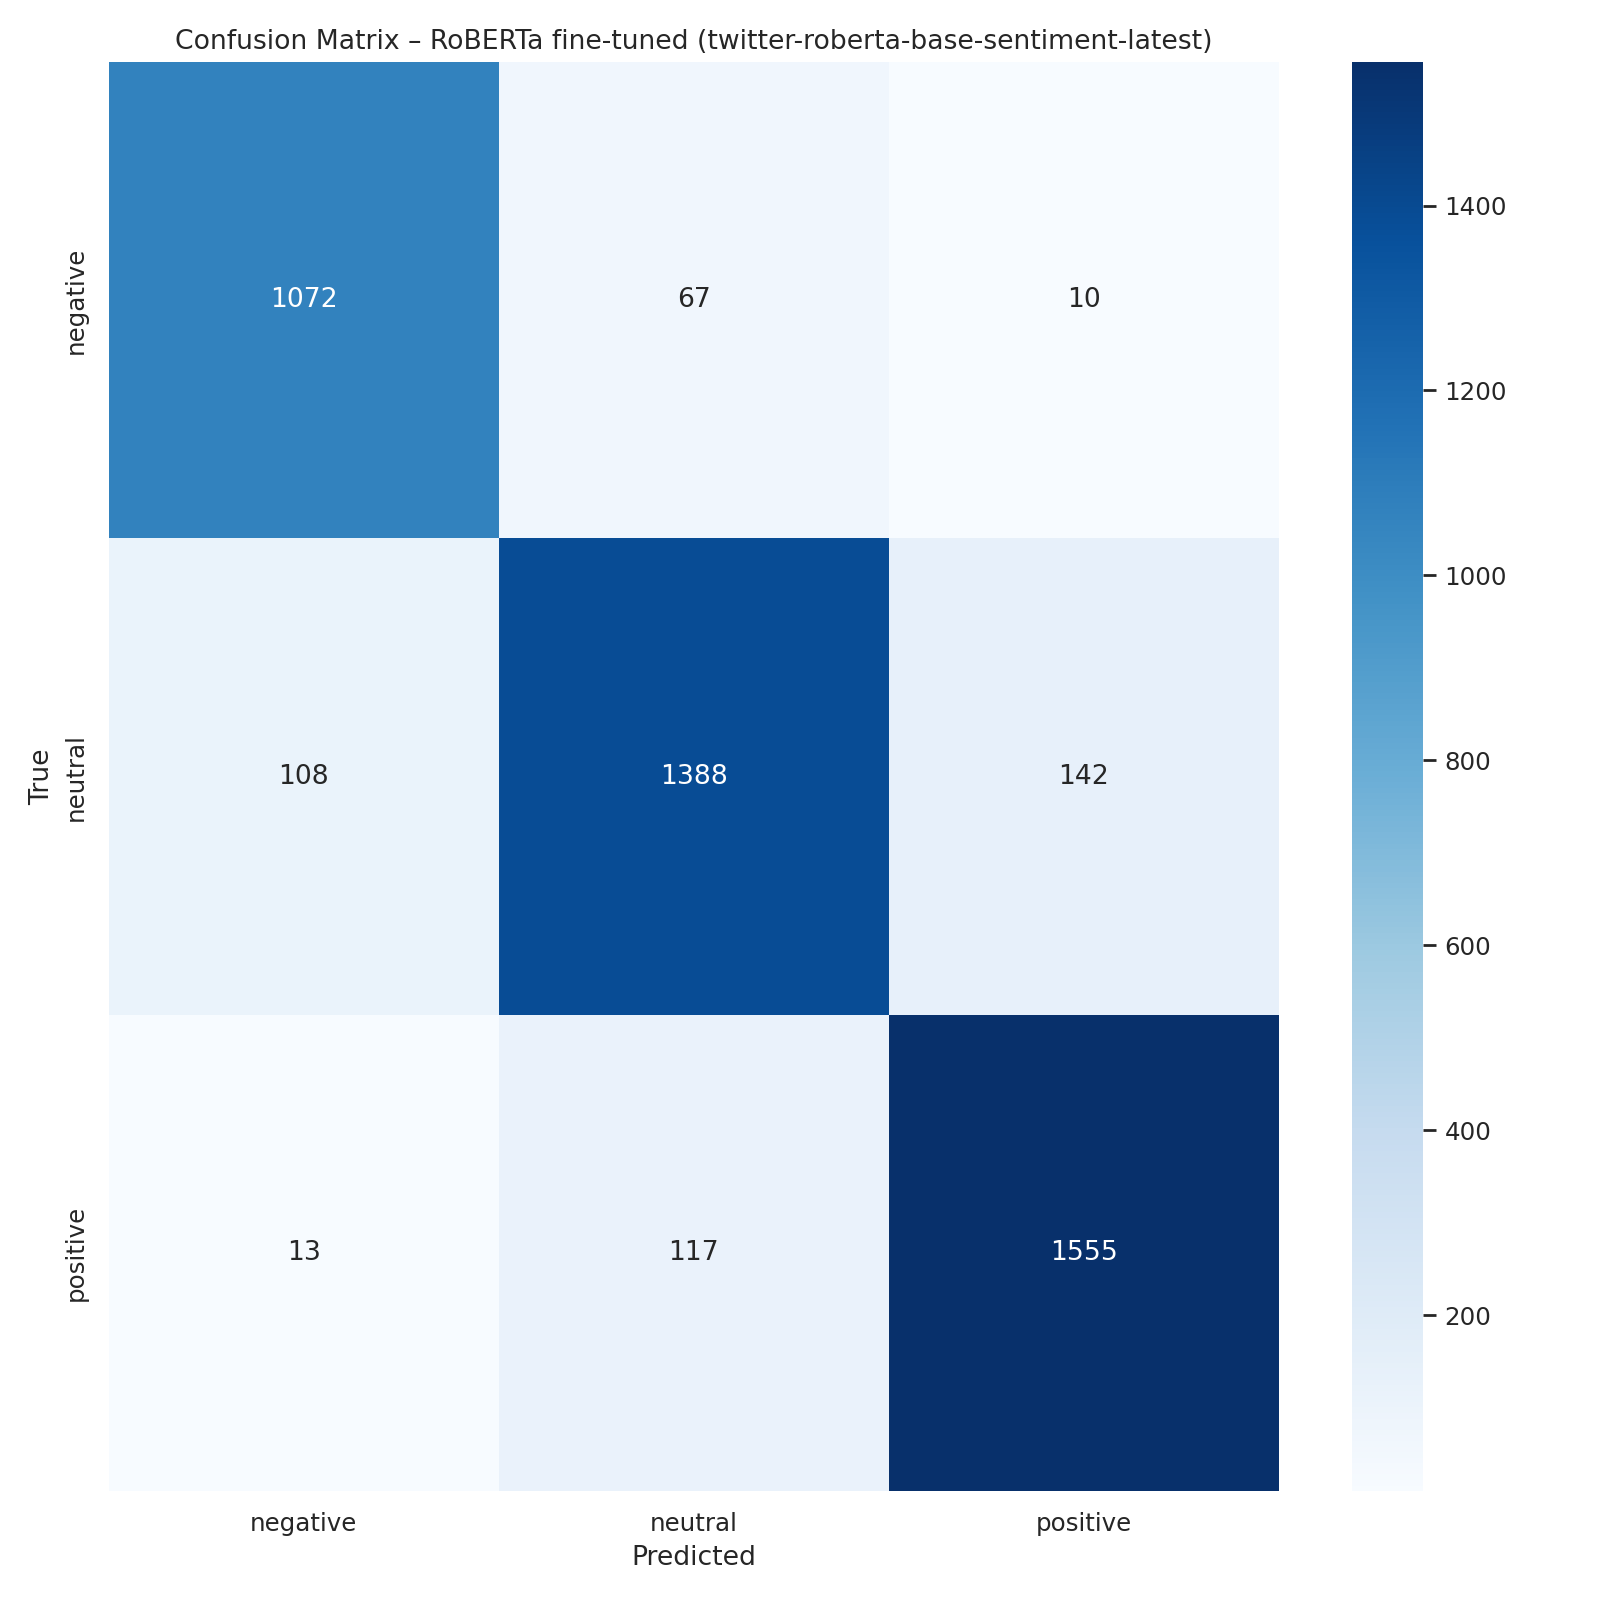
\includegraphics[width=.80\linewidth]{../SCRITPS/artifacts/figures/best_model_cm.png}
  \caption{Confusion matrix for the best model (label order: negative, neutral, positive).}
  \label{fig:best-confusion}
\end{figure}

\begin{table}[H]
  \centering
  \caption{Per-class report of the best model (precision, recall, F1, and support).}
  \label{tab:best-class-report}
  % Generated file; reflects the same label order
  \begin{tabular}{lrrrrrr}
\toprule
class & negative & neutral & positive & accuracy & macro avg & weighted avg \\
\midrule
precision & 0.898575 & 0.882952 & 0.910955 & 0.897809 & 0.897494 & 0.897517 \\
recall & 0.932985 & 0.847375 & 0.922849 & 0.897809 & 0.901070 & 0.897809 \\
f1-score & 0.915457 & 0.864798 & 0.916863 & 0.897809 & 0.899039 & 0.897431 \\
support & 1149.000000 & 1638.000000 & 1685.000000 & 0.897809 & 4472.000000 & 4472.000000 \\
\bottomrule
\end{tabular}

\end{table}

\paragraph{Probability-based curves.}
For models that output class probabilities (e.g., Logistic Regression, Random Forest, CNN, BiLSTM, RoBERTa heads and fine-tuned), we plot macro ROC and macro PR curves that are available in the Repository.\\
The figure below shows the macro ROC curve for the fine-tuned RoBERTa model.
\begin{figure}[H]
  \centering
  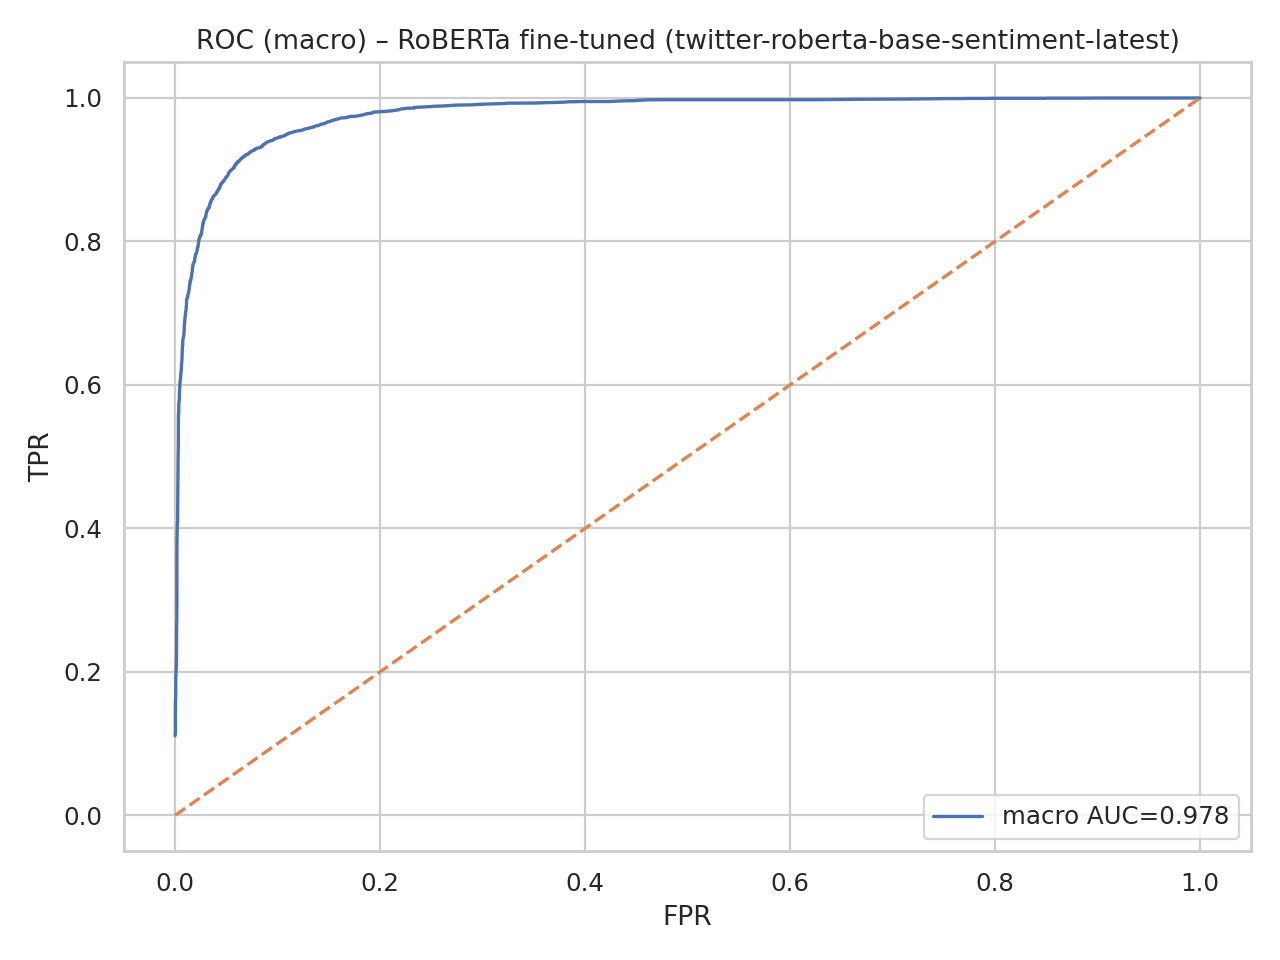
\includegraphics[width=.55\linewidth]{../SCRITPS/artifacts/figures/curves_roberta_fine-tuned_(twitter-roberta-base-sentiment-latest)_roc_macro.png}
  \caption{Macro ROC for a probability-capable model (example: fine-tuned RoBERTa).}
  \label{fig:roc-example}
\end{figure}

\begin{figure}[H]
  \centering
  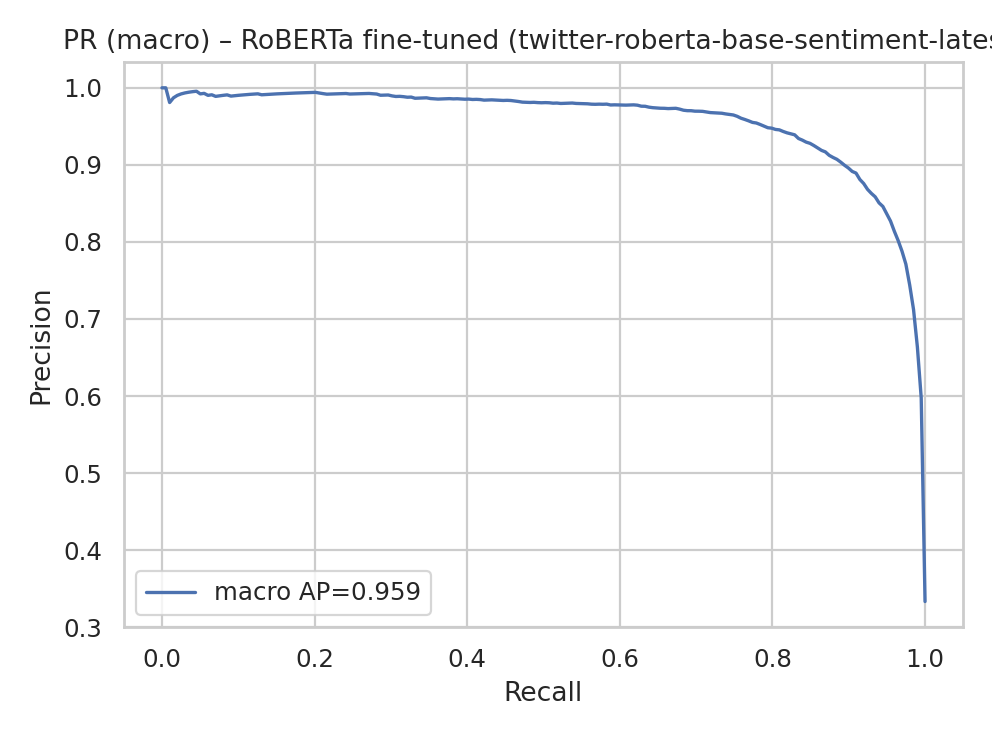
\includegraphics[width=.55\linewidth]{../SCRITPS/artifacts/figures/curves_roberta_fine-tuned_(twitter-roberta-base-sentiment-latest)_pr_macro.png}
  \caption{Macro PR for the same model as Figure~\ref{fig:roc-example}.}
  \label{fig:pr-example}
\end{figure}
The macro ROC curve hugs the top-left corner (AUC $\approx 0.98$), reflecting strong class-averaged discrimination. Across reasonable thresholds, the model attains high true-positive rates at low false-positive rates for most classes.

\paragraph{Training dynamics.}
We report training/validation curves for neural models to show convergence and regularization behavior:
\begin{figure}[H]
  \centering
  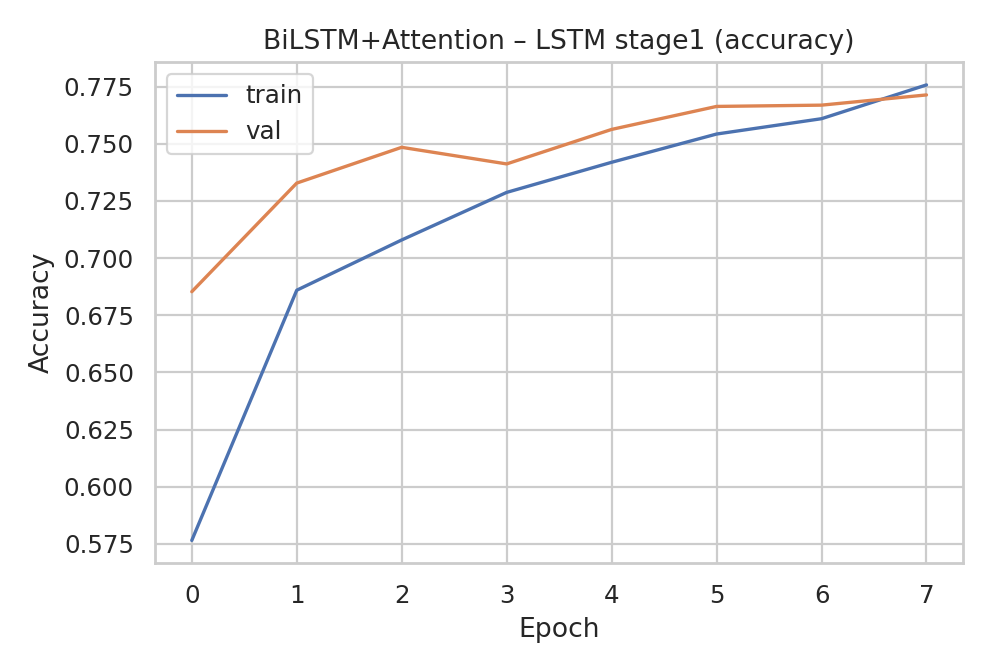
\includegraphics[width=.70\linewidth]{../SCRITPS/artifacts/figures/bilstm+attention_lstm_stage1_acc.png}
  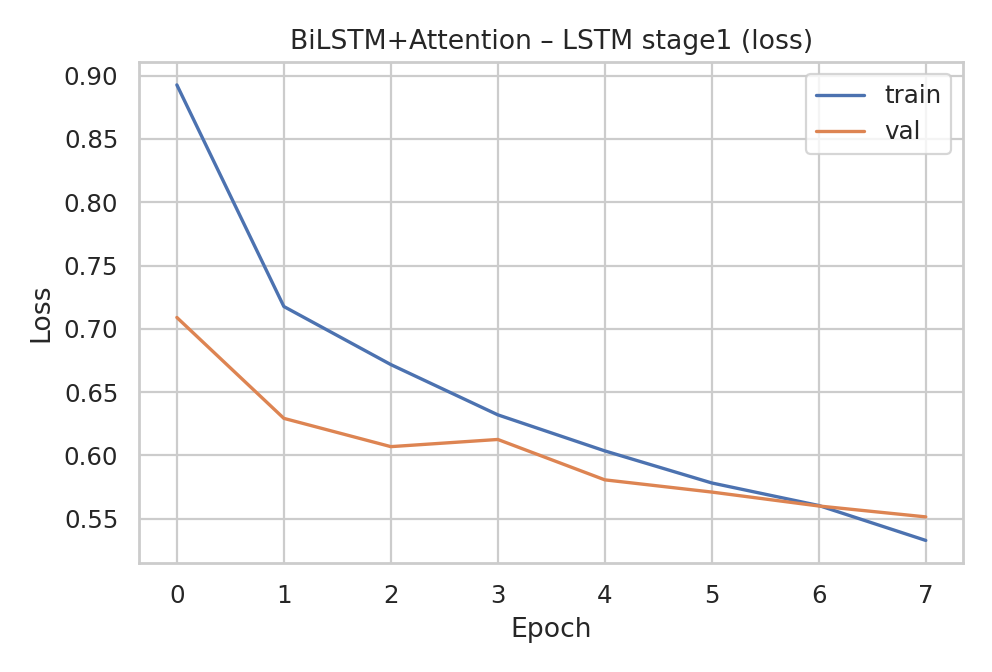
\includegraphics[width=.70\linewidth]{../SCRITPS/artifacts/figures/bilstm+attention_lstm_stage1_loss.png}
  \caption{Example training curves (BiLSTM+Attention). Additional stages/architectures are in the Repository.}
  \label{fig:training-curves}
\end{figure}
Stage-1 learning curves exhibit steady convergence: validation accuracy rises and validation loss falls over epochs. The train–val gap stays small, indicating regularization (dropout/L2) plus early stopping effectively limit overfitting.

\paragraph{Representation analysis}
When using RoBERTa as a frozen feature extractor, we visualize test-set embeddings with UMAP to inspect class separability:
\begin{figure}[H]
  \centering
  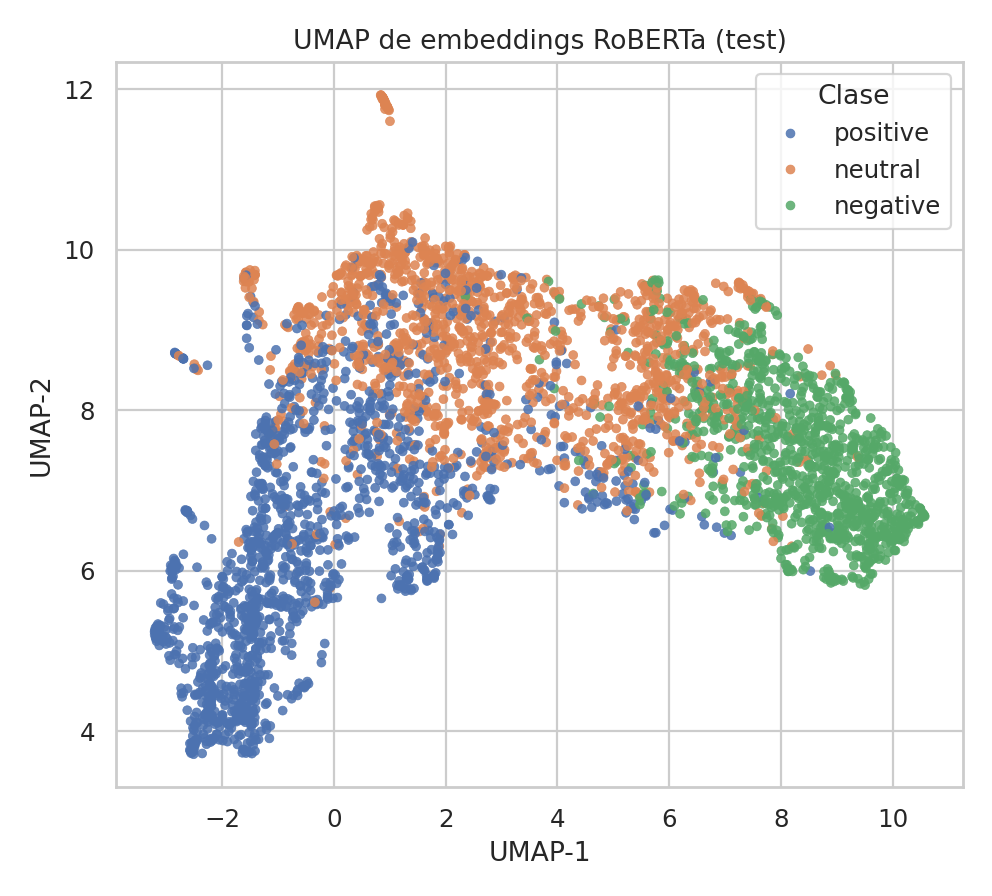
\includegraphics[width=.75\linewidth]{../SCRITPS/artifacts/figures/roberta_fe_test_umap.png}
  \caption{UMAP of mean-pooled RoBERTa embeddings (test split).}
  \label{fig:umap-roberta}
\end{figure}
The UMAP of mean-pooled RoBERTa embeddings on the test set shows well-separated clusters for positive and negative, while neutral occupies a transitional region with more overlap. This suggests the transformer captures polarity clearly, with remaining ambiguity concentrated around the neutral boundary.

\paragraph{Traditional vs.\ deep vs.\ transformers.}
At a glance (Table~\ref{tab:model-comparison}), TF--IDF baselines are lowest (macro-F1 $0.677$--$0.708$), GloVe-based neural models close part of the gap ($0.759$--$0.764$), and transformer variants lead ($0.889$ with frozen RoBERTa + LR; $0.899$ with fine-tuning). Simple voting ensembles ($0.809$) did not outperform the best single model. We keep this section descriptive and defer interpretation to Section~\ref{sec:discussion}.
%%%%%%%%%%%%%%%%%%%%%%%%%%%%%%%%%%%%%%%%%%%%%%%%%%%%%%%%%%%%%%%%%%%%%%%%%%%%%%%%%%%%%%%%%%%%%
\section{Discussion}\label{sec:discussion}

\subsection{Analysis of Results}
Fine-tuned \textbf{RoBERTa} achieved the highest test performance (macro-F1 $=0.899$; Accuracy $0.898$, Precision $0.898$, Recall $0.901$), while using RoBERTa as a frozen feature extractor with a Logistic Regression head was a close second (macro-F1 $=0.889$). The $\approx +1.0$ pp macro-F1 and $+1.2$ pp macro-Recall gains from end-to-end fine-tuning suggest that task-specific adaptation mainly reduces errors on boundary (often \emph{neutral}) tweets. Non-transformer neural models (BiLSTM+Attention $0.764$, CNN with SE+Attn $0.759$) clearly outperform TF--IDF baselines (Logistic Regression $0.708$, LinearSVC $0.699$, Random Forest $0.677$) but still trail transformers, consistent with the limits of static word embeddings and shallower context modeling. Confusion matrices (Fig.~\ref{fig:best-confusion}) and the UMAP projection (Fig.~\ref{fig:umap-roberta}) indicate that residual confusion is concentrated around the \emph{neutral} region.
Both ensemble variants (weighted and majority voting) reached macro-F1 $=0.809$, below the best single transformer. Operationally, the frozen RoBERTa + LR head offers a strong accuracy--latency trade-off, whereas fine-tuning yields a small but reliable boost at higher compute cost.

\subsection{Strengths and Weaknesses}
\paragraph{Strengths.} 
(i) A Twitter-aware preprocessing pipeline preserves emojis/emoticons and hashtag semantics; (ii) the study spans three modeling families (TF--IDF, GloVe-based neural, transformers) for a fair comparison; (iii) careful training (class weights, staged unfreezing, cosine restarts) stabilizes neural models; (iv) full reproducibility: seeds, cached embeddings, and exported artifacts (tables/figures).
\paragraph{Weaknesses.}
(i) The naive voting ensembles (fixed weights/majority) underperformed the best single transformer, indicating limited error complementarity or poor weighting; (ii) compute cost: transformer fine-tuning is heavier than TF--IDF/Glove baselines.

\subsection{Limitations}
This study has several limitations. First, labels are derived from \texttt{cardiffnlp/twitter-roberta-base-sentiment-latest}, which we also use as a backbone; this ``teacher--student'' setup can bias evaluation toward transformer variants that approximate the teacher's decision boundary. Second, the dataset covers only the first day of the tournament, limiting topical and temporal diversity. Third, global tweets are likely multilingual, while this study worked in English, it may not perform in the same way with other languages.

\paragraph{Compute constraints.}
We trained under limited GPU memory and time on a single device, which constrained batch sizes, sequence lengths, and training schedules. Consequently, we could not run extensive hyperparameter sweeps or multi-seed cross-validation, nor explore larger backbones (e.g., RoBERTa-large, DeBERTa-v3-large, XLM-Roberta large), longer-context inputs, or calibration-aware/stacked ensembles. These restrictions likely cap absolute performance and stability, so the reported scores should be viewed as conservative lower bounds.

\subsection{Future Work}
(i) Evaluate cross-domain generalization (other tournament days, clubs, other sports) and cross-lingual robustness (e.g., XLM-T, mDeBERTa, or multilingual RoBERTa); (iii) replace naive voting with calibrated stacking: temperature scaling/Platt scaling per model, then a meta-learner on per-class probabilities; (iv) ablations on preprocessing (emoji/hashtag handling), sequence length, and embedding choices; (v) explore larger or instruction-tuned transformers and prompt-based zero-/few-shot setups; (vi) address \emph{neutral} with margin-aware losses or focal loss and targeted augmentation for borderline cases.

\subsection{Concluding Remarks}
Our study confirms the advantage of transformer-based representations for Twitter sentiment: most gains stem from domain-pretrained RoBERTa features, with fine-tuning providing a small but reliable boost—particularly on ambiguous tweets. Classic TF--IDF and GloVe-based neural models remain competitive as efficient baselines, yet they struggle on \emph{neutral}.\\
Future work should prioritize cross-sports-domain and cross-lingual generalization, calibration-aware stacking over naive voting, systematic ablations of preprocessing/sequence length/embeddings, scaling to larger or instruction-tuned transformers and prompt-based zero/few-shot setups, and strengthening the \emph{neutral} boundary via margin-aware or focal losses with targeted augmentation.
%%%%%%%%%%%%%%%%%%%%%%%%%%%%%%%%%%%%%%%%%%%%%%%%%%%%%%%%%%%%%%%%%%%%%%%%%%%%%%%%%%%%%%%%%%%%%
\begin{thebibliography}{9}
\bibitem{ref1} Barnaghi, P., Ghaffari, P., \& Breslin, J. (2016). Opinion mining and sentiment polarity on Twitter and correlation between events and sentiment. \textit{Journal of Web Semantics}, 30, 1–11.
\bibitem{ref2} Venkatesh, K., et al. (2019). Deep learning-based hybrid CNN-LSTM model for sentiment classification on sports tweets. \textit{Procedia Computer Science}, 152, 341–348.
\bibitem{ref3} Barbieri, F., Camacho-Collados, J., Neves, L., \& Espinosa Anke, L. (2020). TweetEval: Unified benchmark and comparative evaluation for tweet classification. \textit{Proceedings of EMNLP 2020}, 1644–1650.
\bibitem{ref4} Fadel, A., et al. (2023). Fine-tuning RoBERTa for sentiment analysis of sports-related tweets. \textit{IEEE Transactions on Affective Computing}, 14(2), 1–12.
\bibitem{ref5}  
Barnaghi, P., Ghaffari, P., \& Breslin, J. G. (2015). Text Analysis and Sentiment Polarity on FIFA World Cup 2014 Tweets. En *Proceedings of the KDD’15 Workshop on Large-Scale Sports Analytics*.  
\end{thebibliography}
%%%%%%%%%%%%%%%%%%%%%%%%%%%%%%%%%%%%%%%%%%%%%%%%%%%%%%%%%%%%%%%%%%%%%%%%%%%%%%%%%%%%%%%%%%%%%
\section{Appendix}
\subsection{GitHub Repository}
\url{https://github.com/enriquegomeztagle/MCD-NLP-SentimentAnalysisOfFIFATweets-FinalProject}
%%%%%%%%%%%%%%%%%%%%%%%%%%%%%%%%%%%%%%%%%%%%%%%%%%%%%%%%%%%%%%%%%%%%%%%%%%%%%%%%%%%%%%%%%%%%%
\end{document}
